\section{Referencia de la Clase Albaranes\-Proveedor\-List\-Subform}
\label{classAlbaranesProveedorListSubform}\index{AlbaranesProveedorListSubform@{AlbaranesProveedorListSubform}}
Clase que maneja el detalle de los albaranes de proveedor.  


{\tt \#include $<$albaranesproveedor.h$>$}

Diagrama de herencias de Albaranes\-Proveedor\-List\-Subform\begin{figure}[H]
\begin{center}
\leavevmode
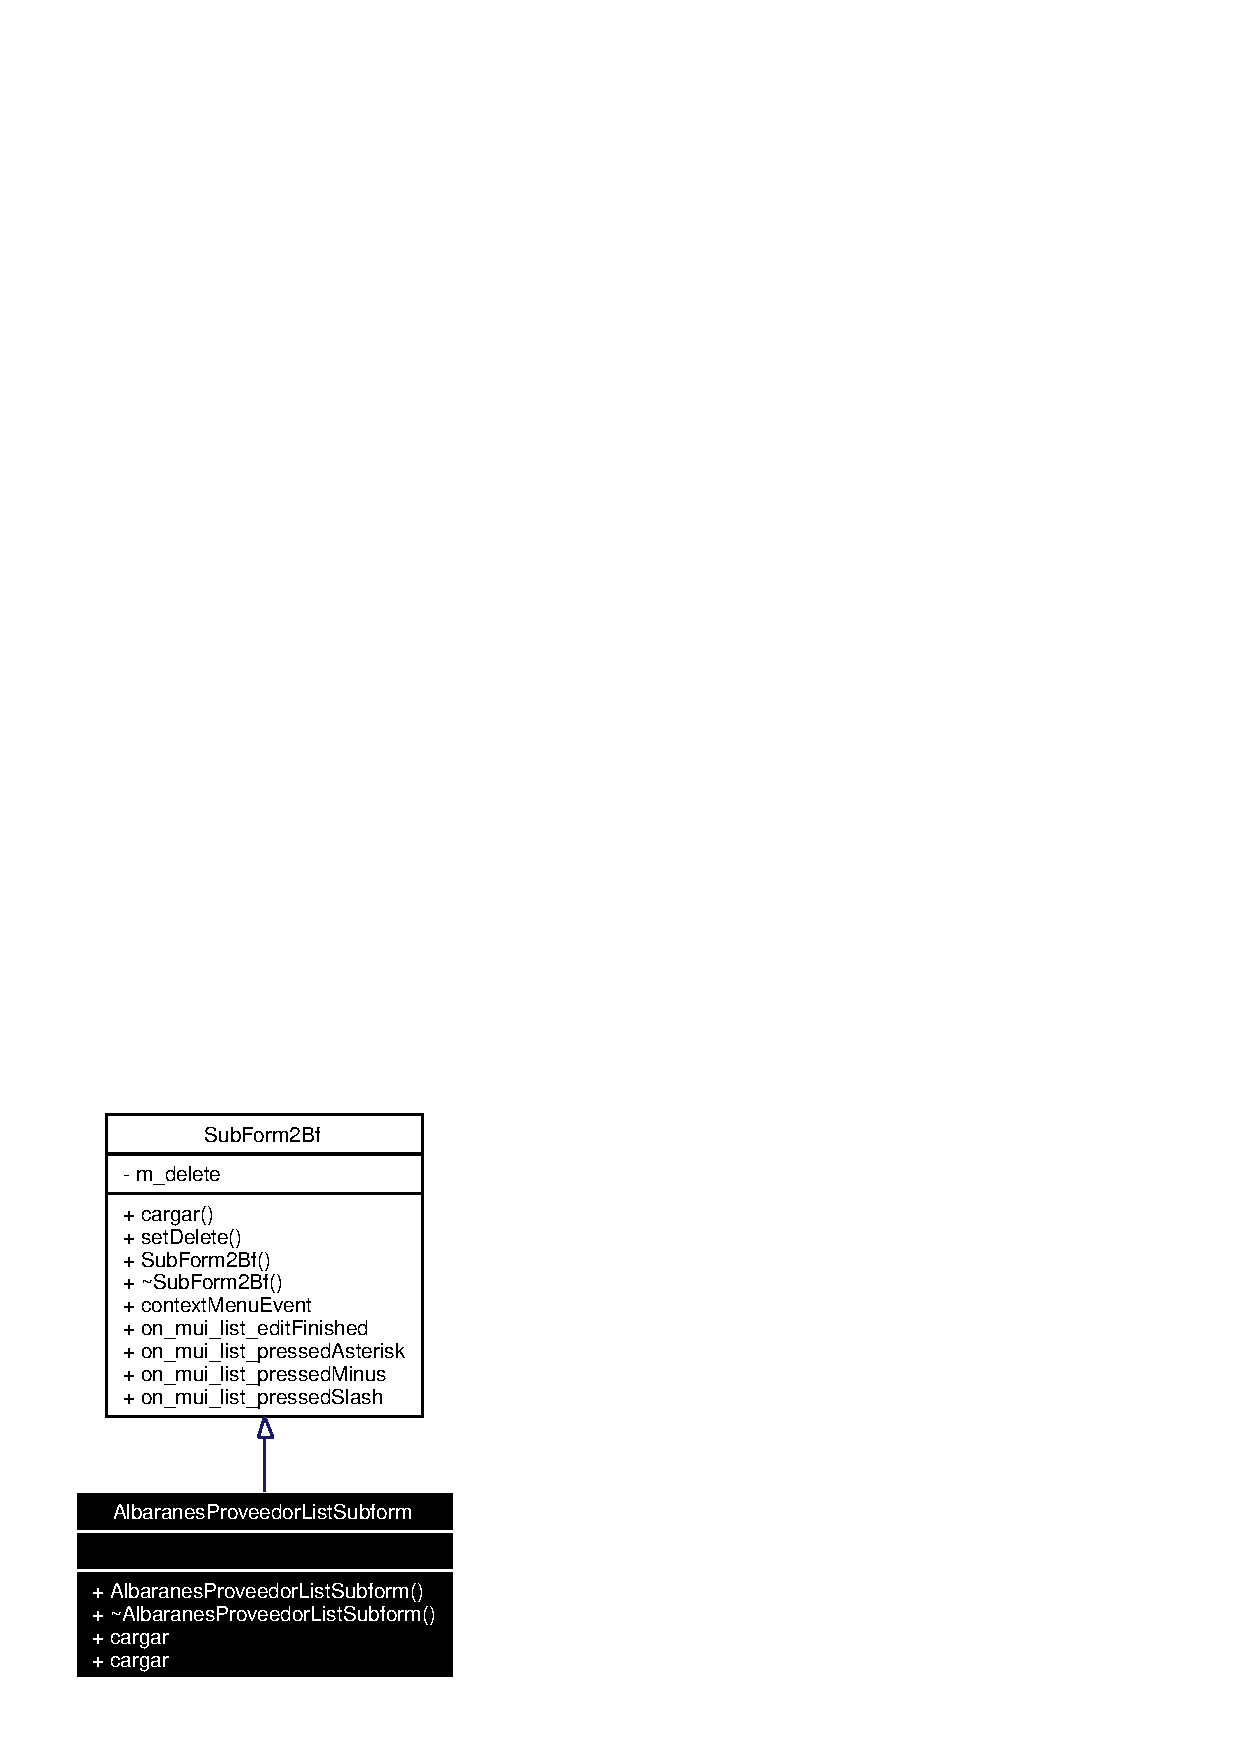
\includegraphics[width=109pt]{classAlbaranesProveedorListSubform__inherit__graph}
\end{center}
\end{figure}
Diagrama de colaboraci\'{o}n para Albaranes\-Proveedor\-List\-Subform:\begin{figure}[H]
\begin{center}
\leavevmode
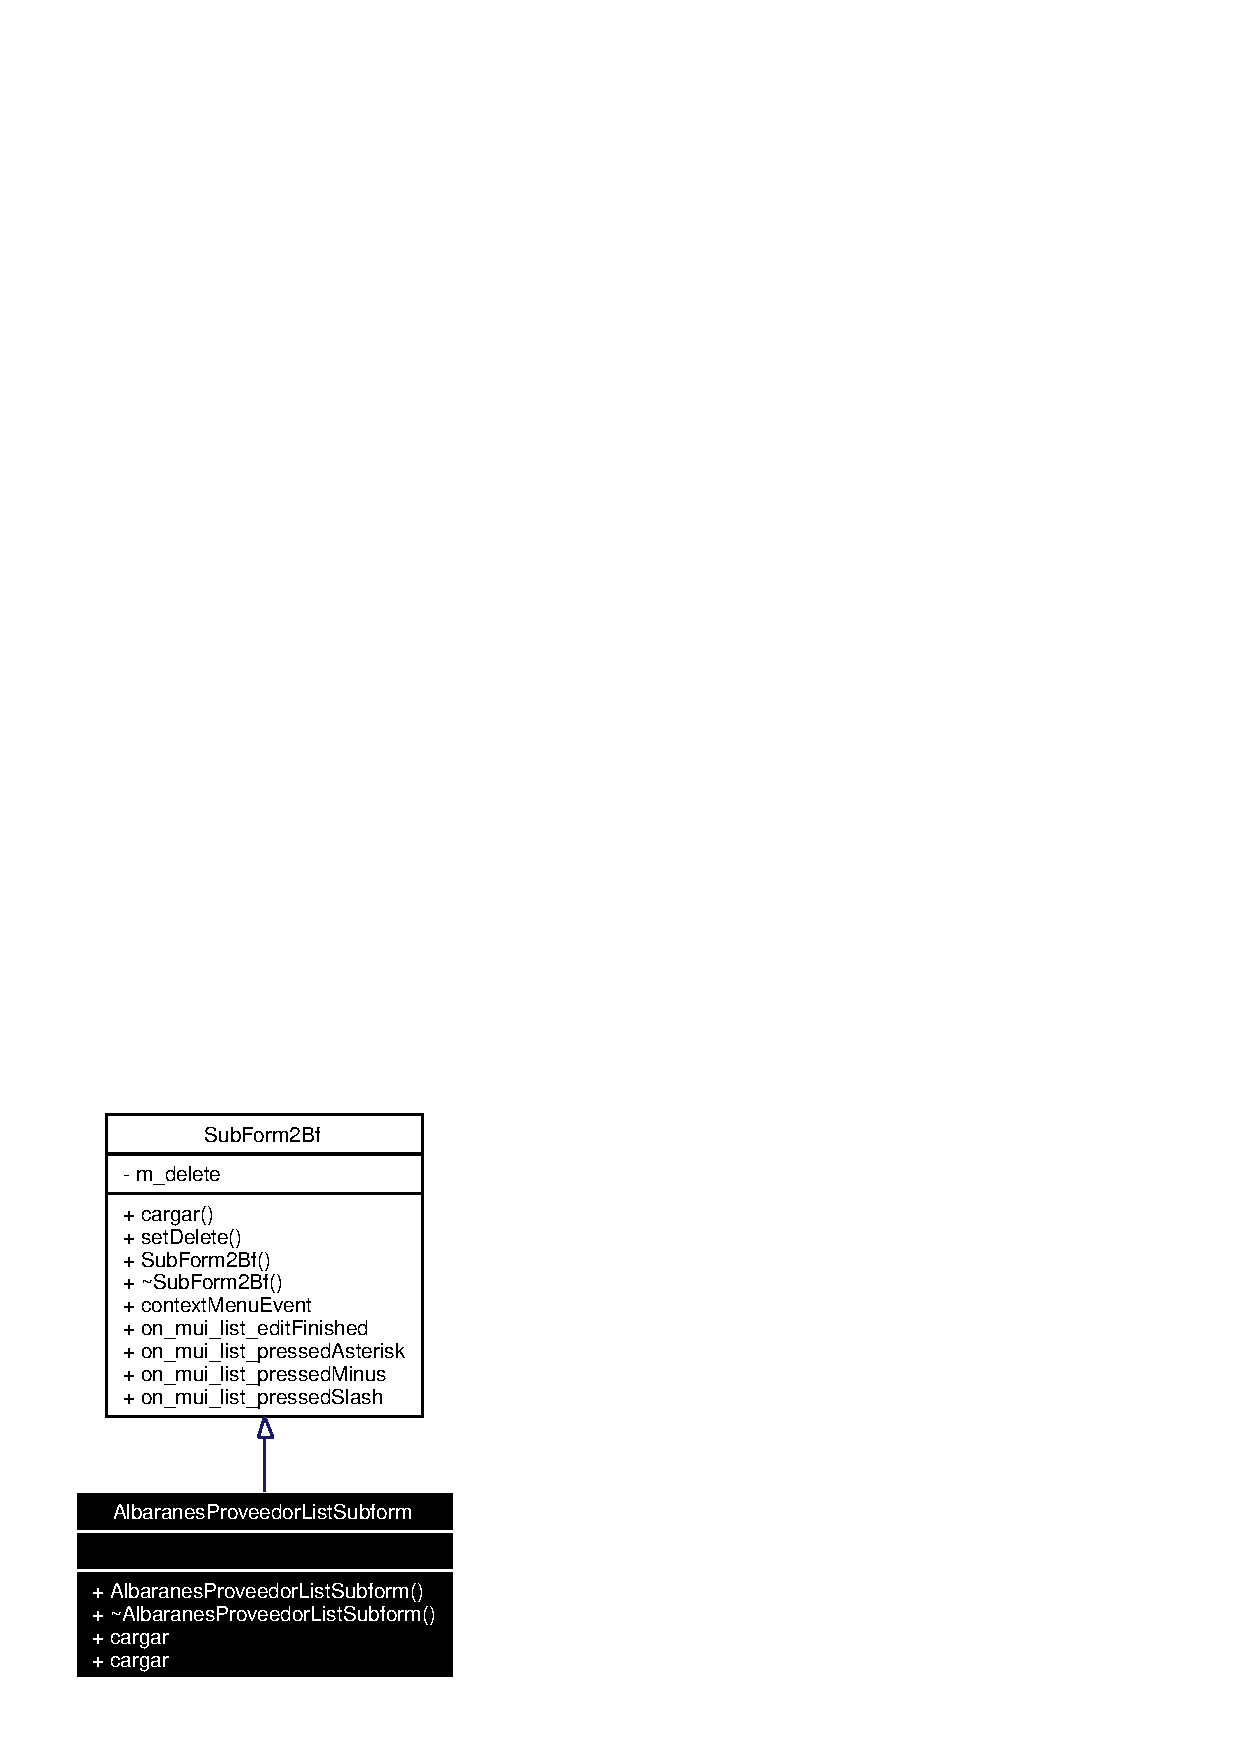
\includegraphics[width=109pt]{classAlbaranesProveedorListSubform__coll__graph}
\end{center}
\end{figure}
\subsection*{Slots p\'{u}blicos}
\begin{CompactItemize}
\item 
virtual void {\bf cargar} (QString query)\label{classAlbaranesProveedorListSubform_i0}

\item 
virtual void {\bf cargar} ()\label{classAlbaranesProveedorListSubform_i1}

\end{CompactItemize}
\subsection*{M\'{e}todos p\'{u}blicos}
\begin{CompactItemize}
\item 
{\bf Albaranes\-Proveedor\-List\-Subform} (QWidget $\ast$parent=0)
\end{CompactItemize}


\subsection{Descripci\'{o}n detallada}
Clase que maneja el detalle de los albaranes de proveedor. 



\subsection{Documentaci\'{o}n del constructor y destructor}
\index{AlbaranesProveedorListSubform@{Albaranes\-Proveedor\-List\-Subform}!AlbaranesProveedorListSubform@{AlbaranesProveedorListSubform}}
\index{AlbaranesProveedorListSubform@{AlbaranesProveedorListSubform}!AlbaranesProveedorListSubform@{Albaranes\-Proveedor\-List\-Subform}}
\subsubsection{\setlength{\rightskip}{0pt plus 5cm}Albaranes\-Proveedor\-List\-Subform::Albaranes\-Proveedor\-List\-Subform (QWidget $\ast$ {\em parent} = {\tt 0})}\label{classAlbaranesProveedorListSubform_a0}


============================================================================= SUBFORMULARIO ============================================================================= 

La documentaci\'{o}n para esta clase fu\'{e} generada a partir de los siguientes archivos:\begin{CompactItemize}
\item 
albaranesproveedor.h\item 
albaranesproveedor.cpp\end{CompactItemize}
